\begin{figure}
\centering
\begin{tabular}{ccc}
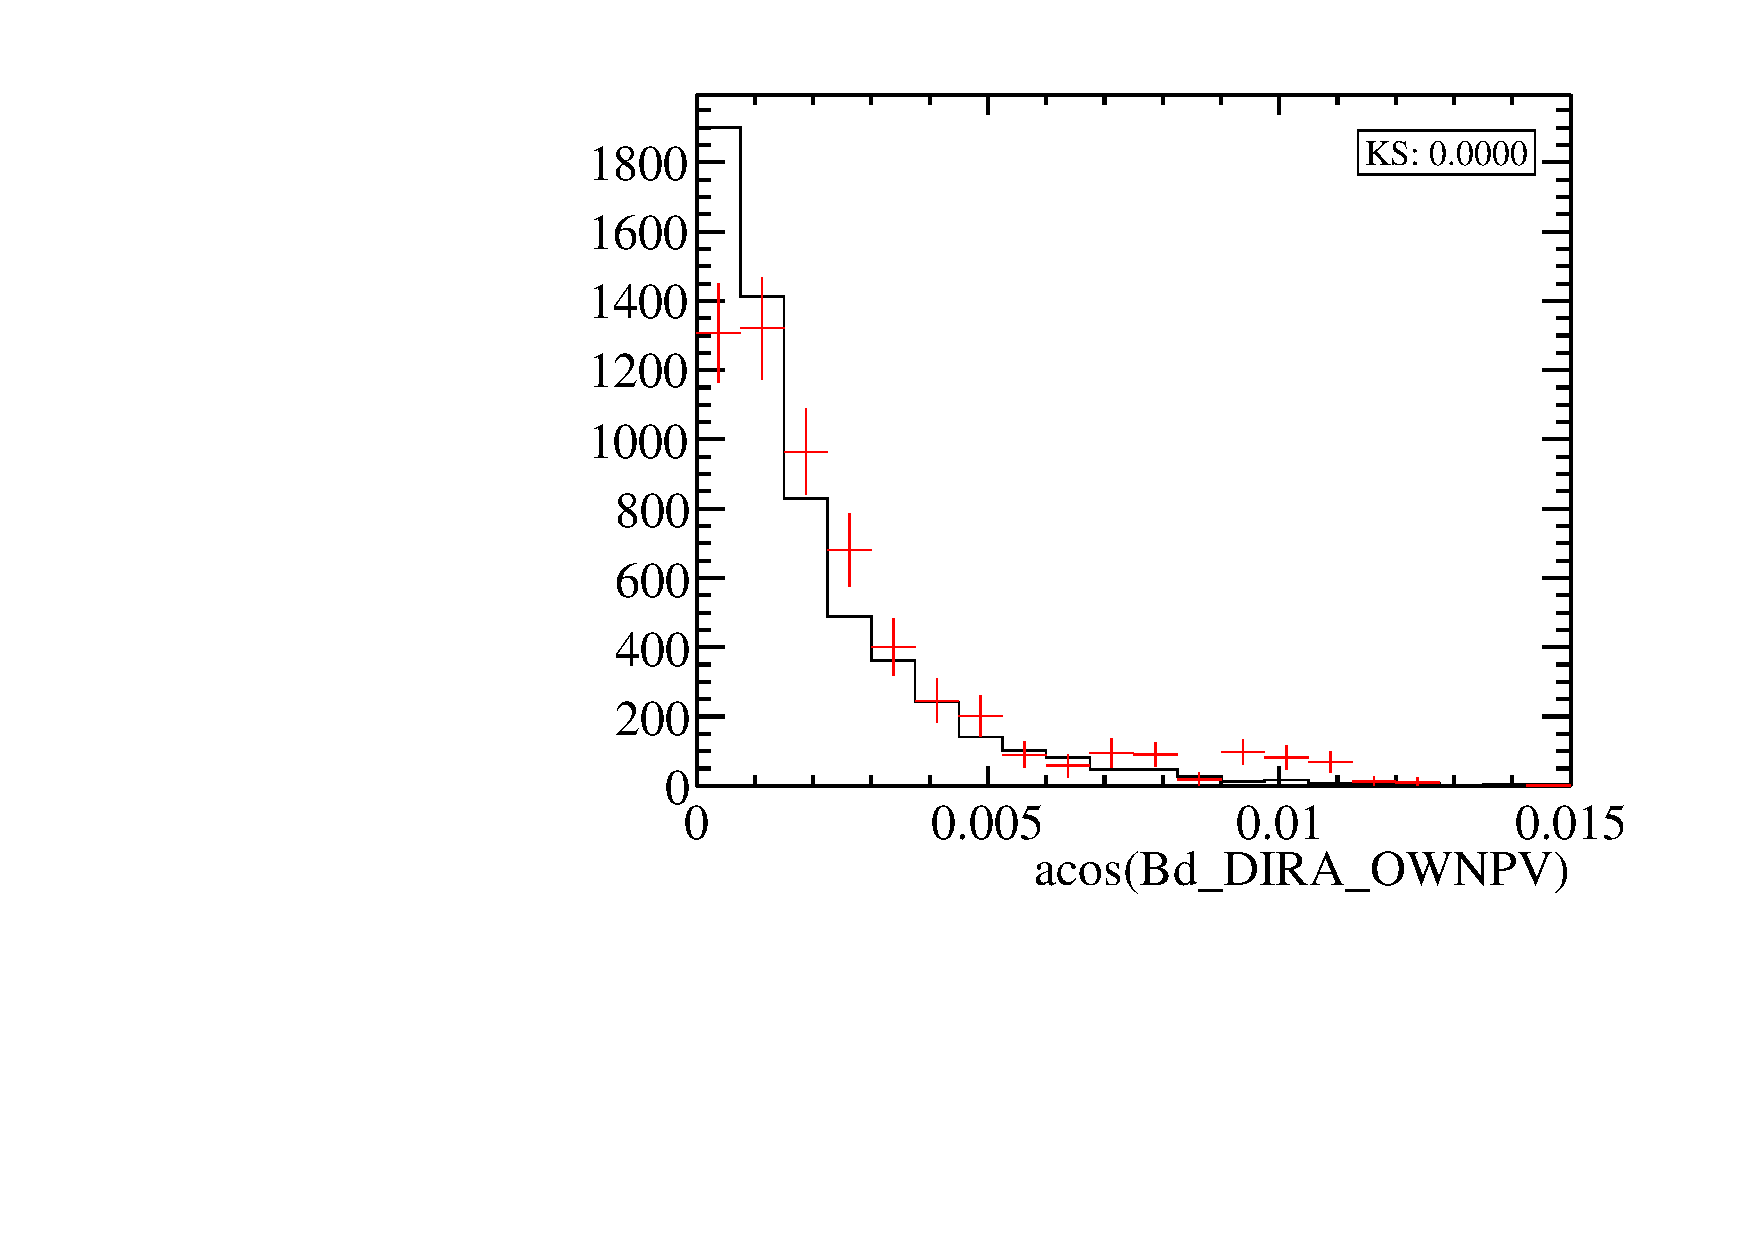
\includegraphics[width=0.3\textwidth]{ANA_resources/Plots/Monte_carlo/data_vs_MC/Kpi/acos(Bd_DIRA_OWNPV)_2012.pdf} & 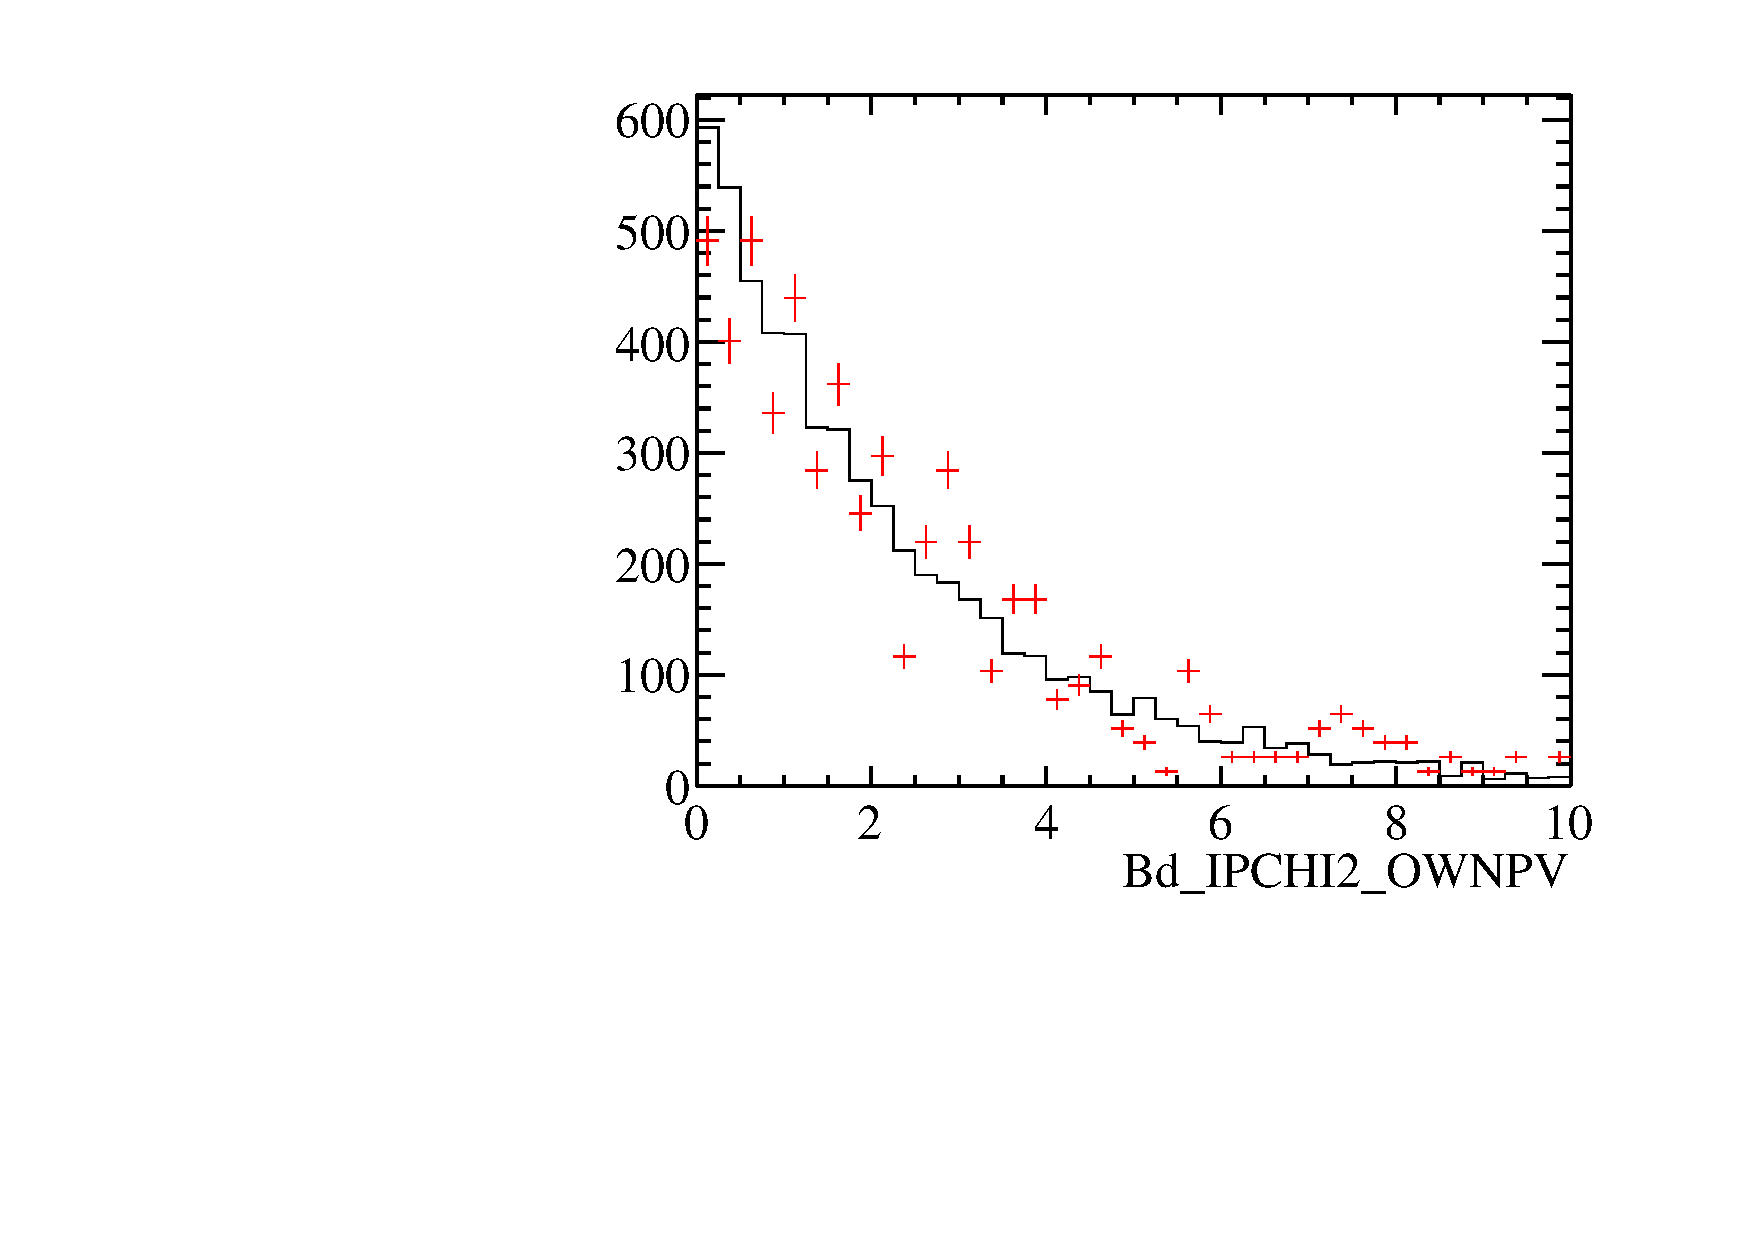
\includegraphics[width=0.3\textwidth]{ANA_resources/Plots/Monte_carlo/data_vs_MC/Kpi/Bd_IPCHI2_OWNPV_2012.pdf} & 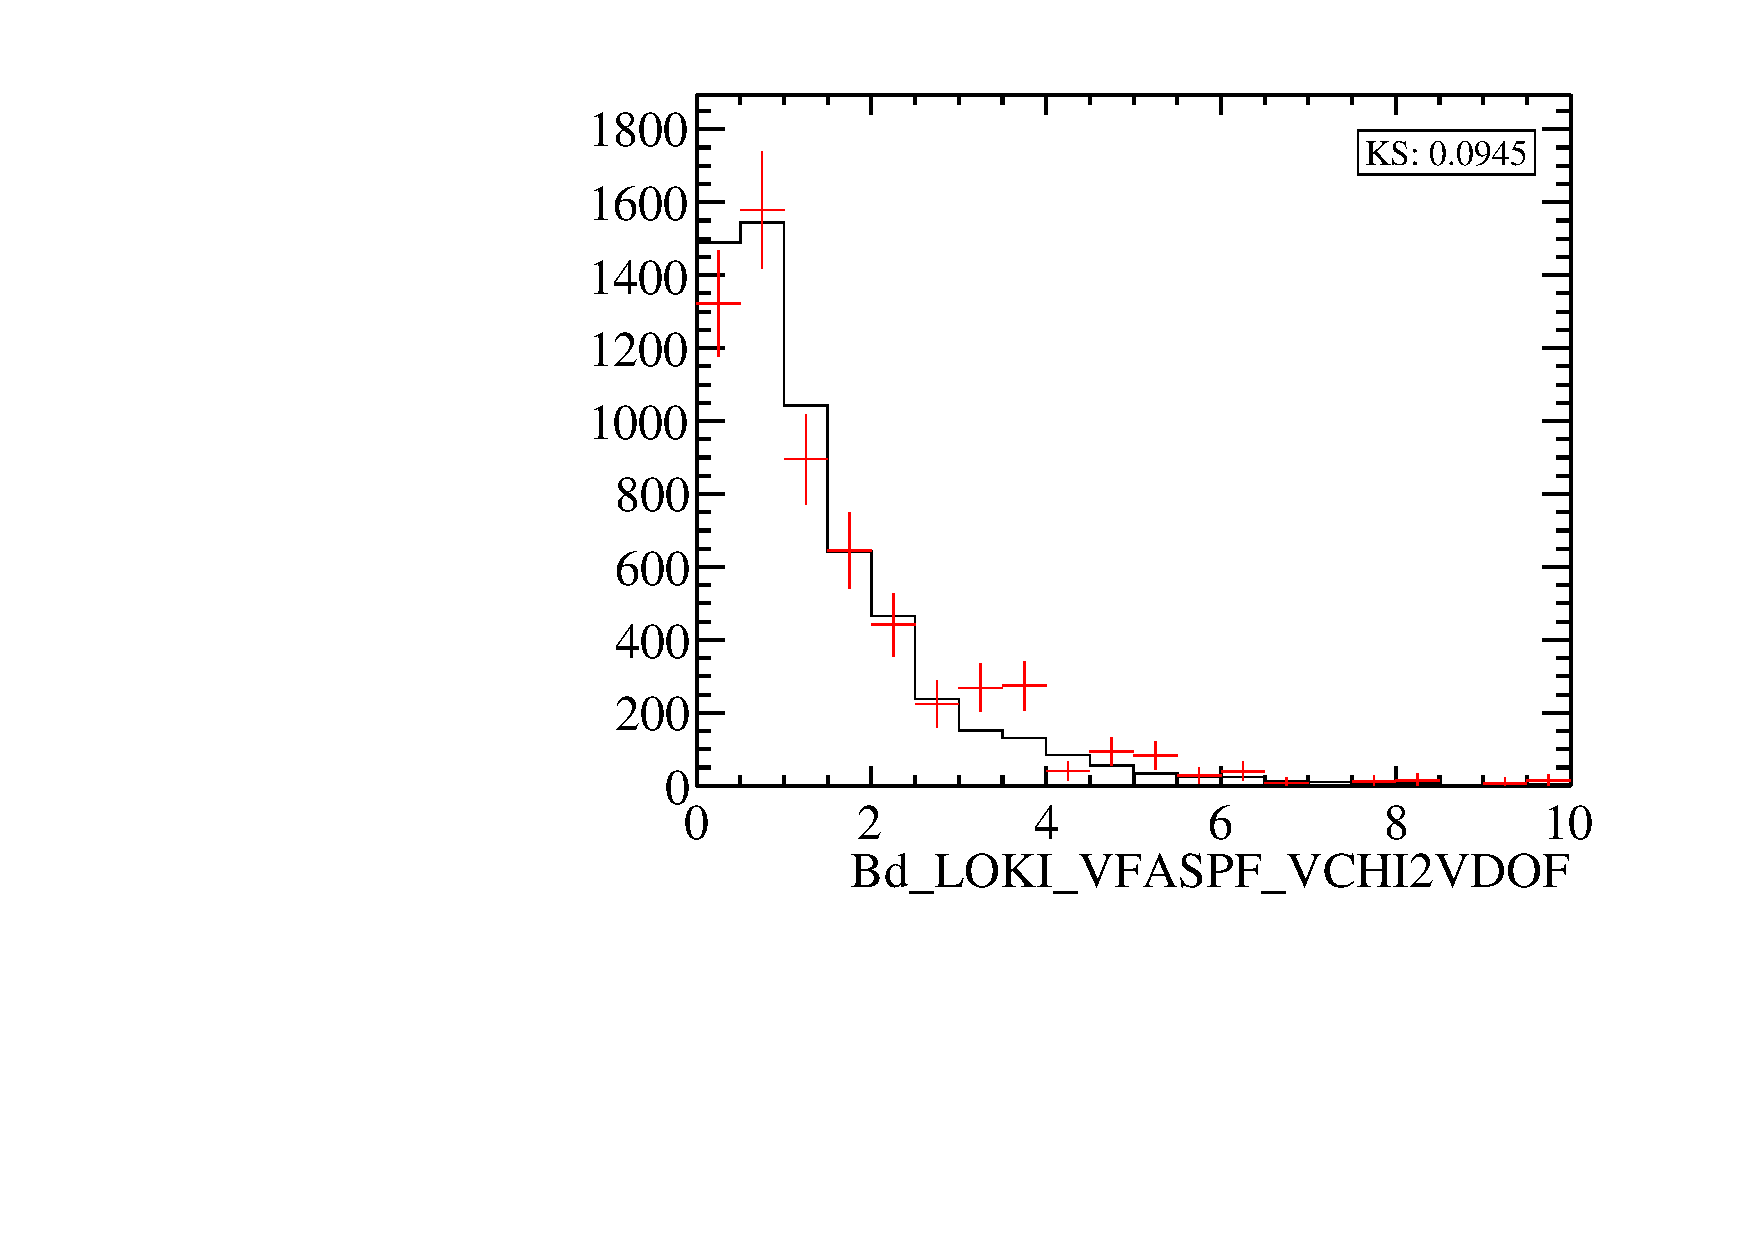
\includegraphics[width=0.3\textwidth]{ANA_resources/Plots/Monte_carlo/data_vs_MC/Kpi/Bd_LOKI_VFASPF_VCHI2VDOF_2012.pdf} \\
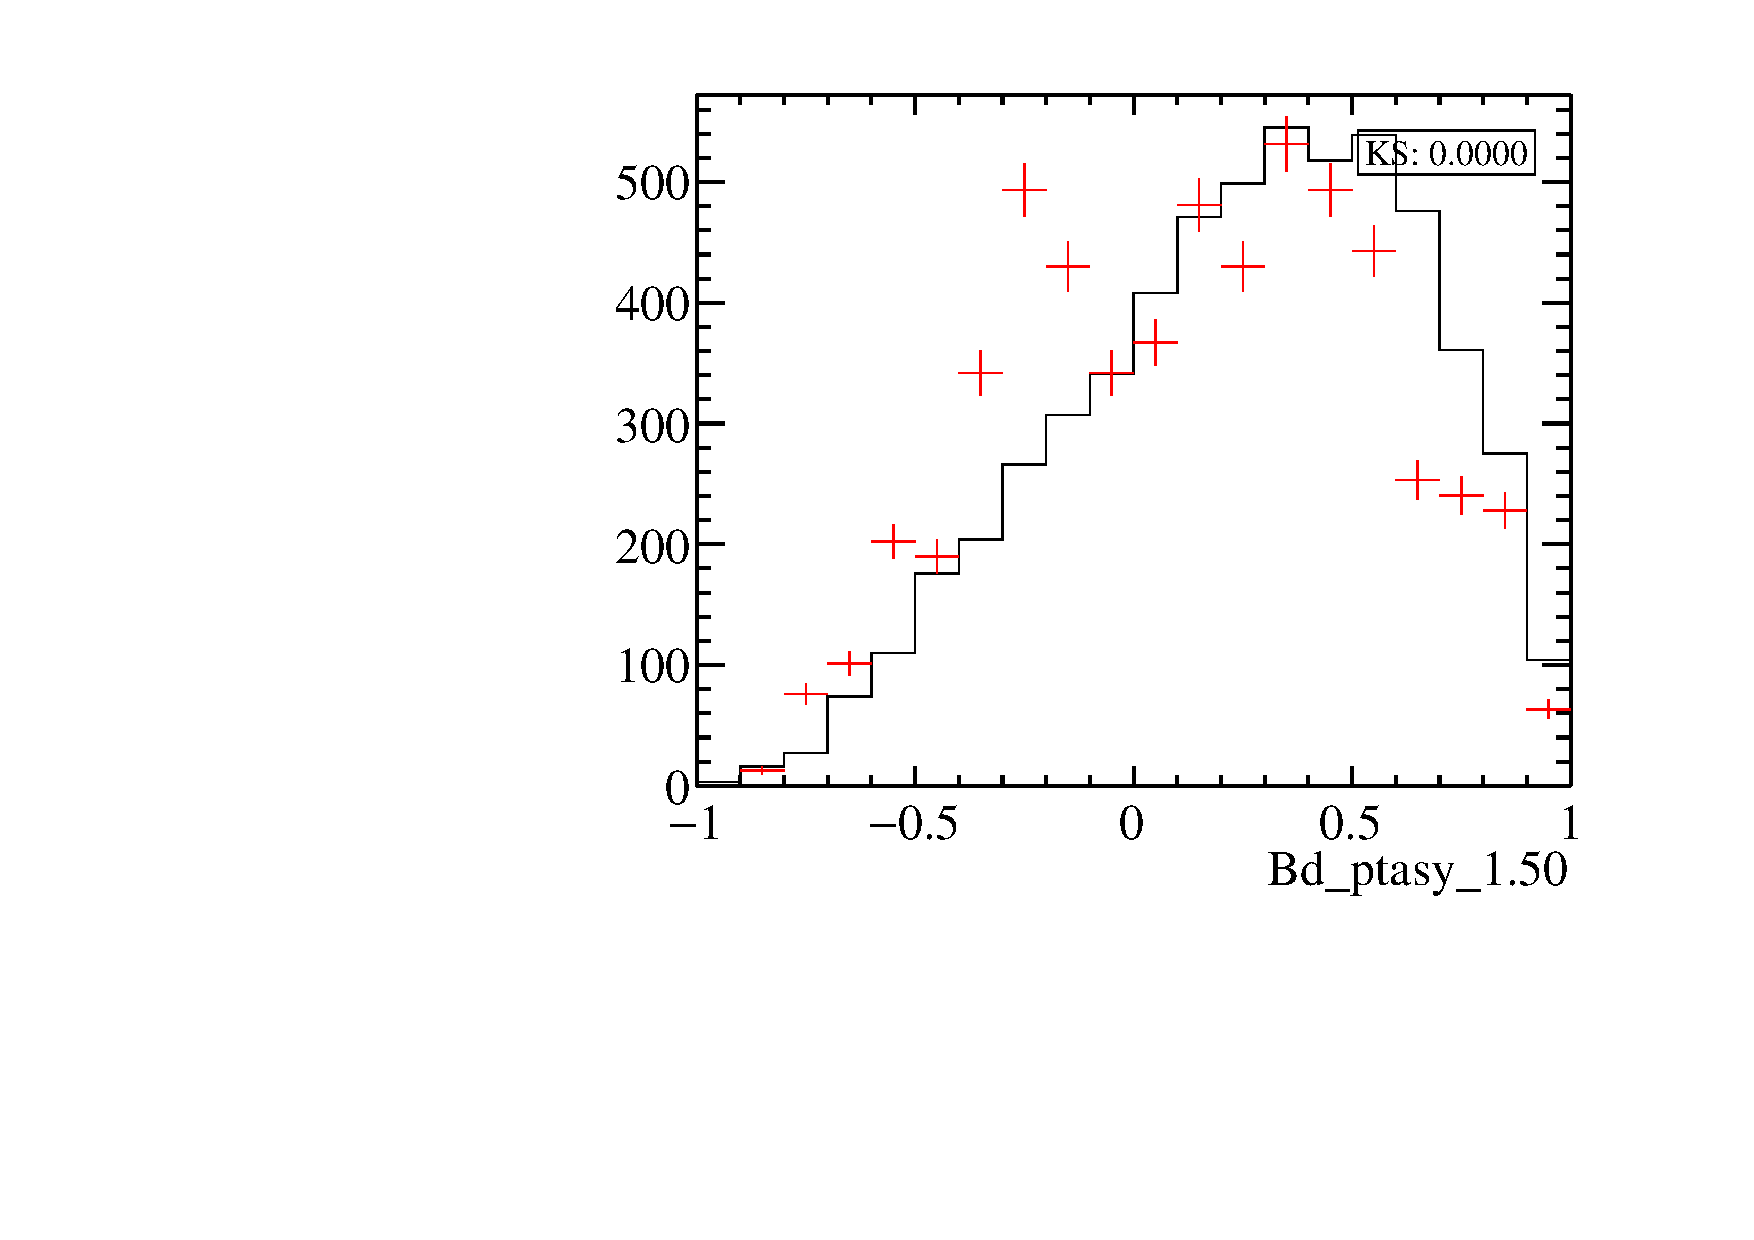
\includegraphics[width=0.3\textwidth]{ANA_resources/Plots/Monte_carlo/data_vs_MC/Kpi/Bd_ptasy_1_50_2012.pdf} & 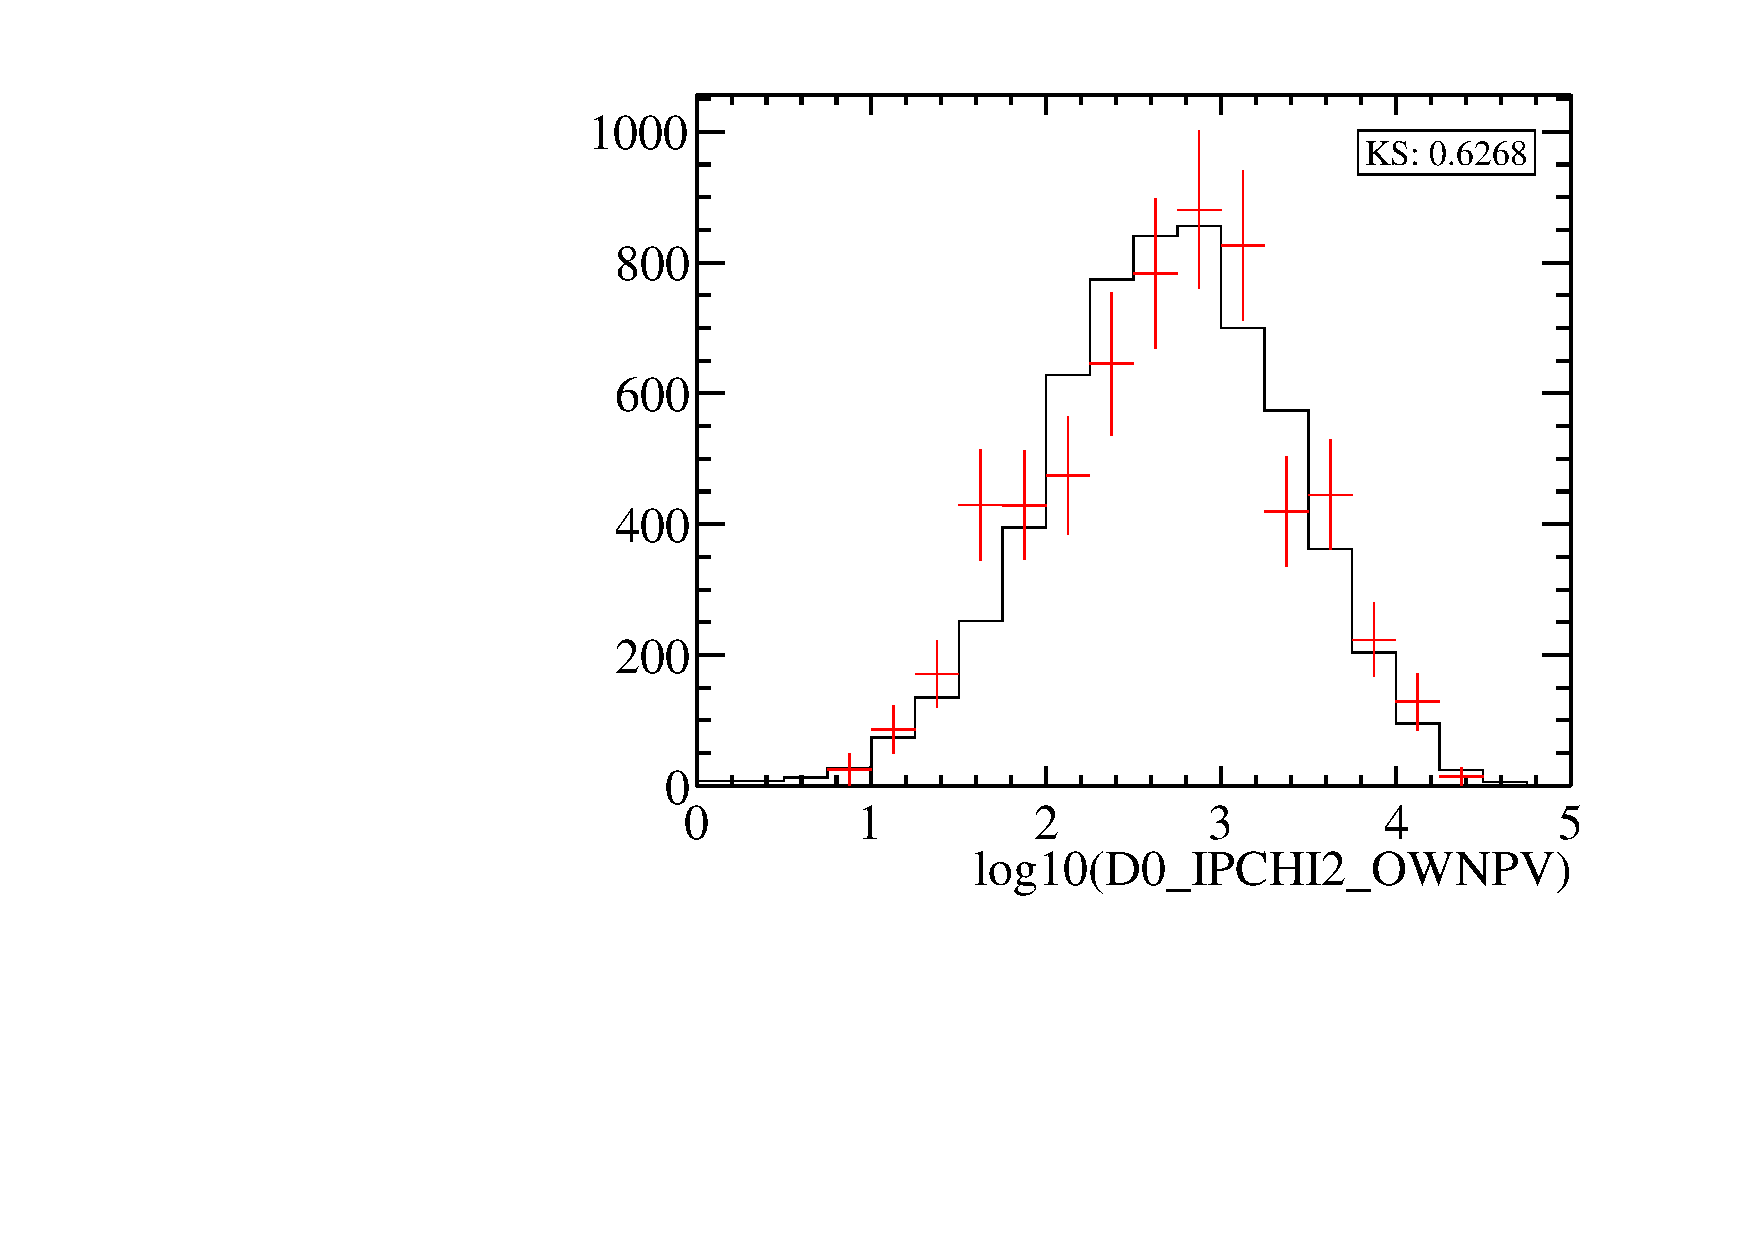
\includegraphics[width=0.3\textwidth]{ANA_resources/Plots/Monte_carlo/data_vs_MC/Kpi/log10(D0_IPCHI2_OWNPV)_2012.pdf} & 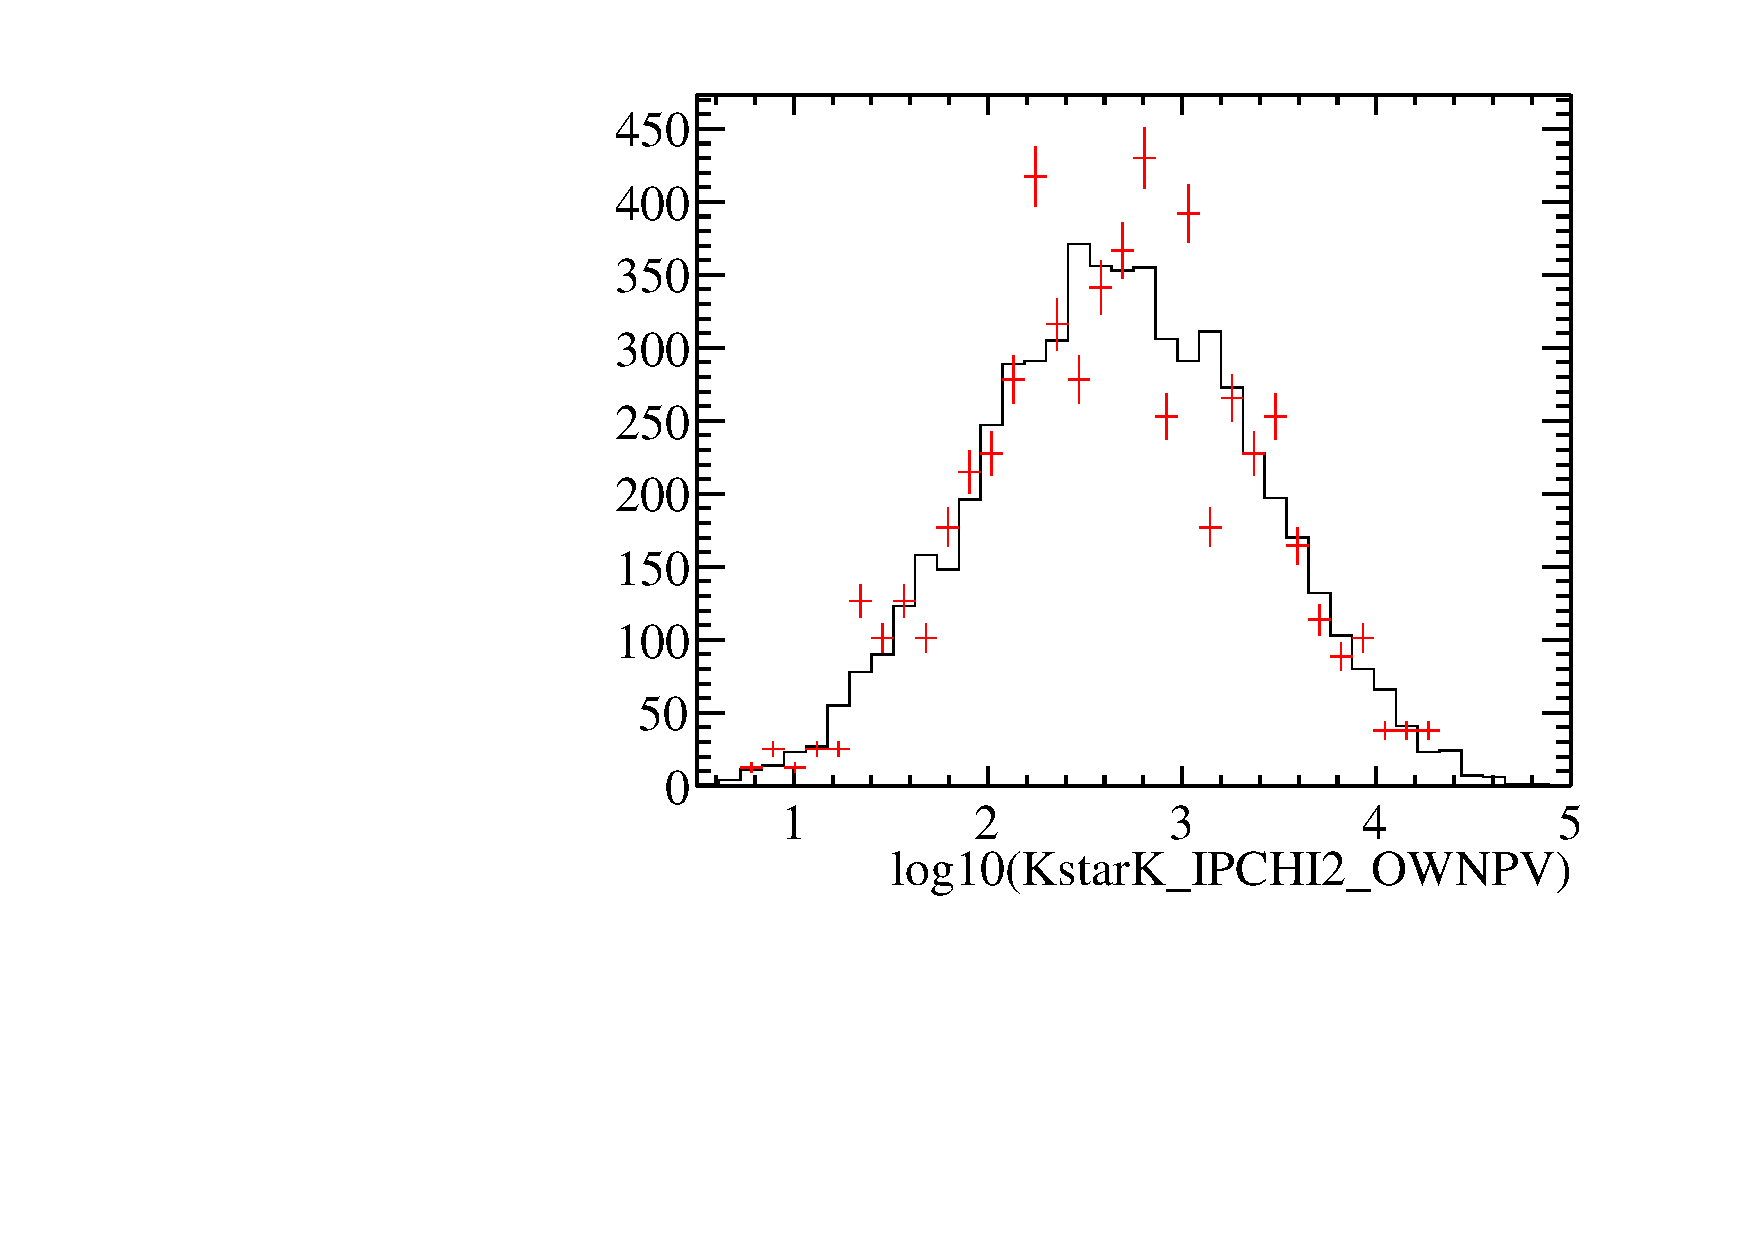
\includegraphics[width=0.3\textwidth]{ANA_resources/Plots/Monte_carlo/data_vs_MC/Kpi/log10(KstarK_IPCHI2_OWNPV)_2012.pdf} \\
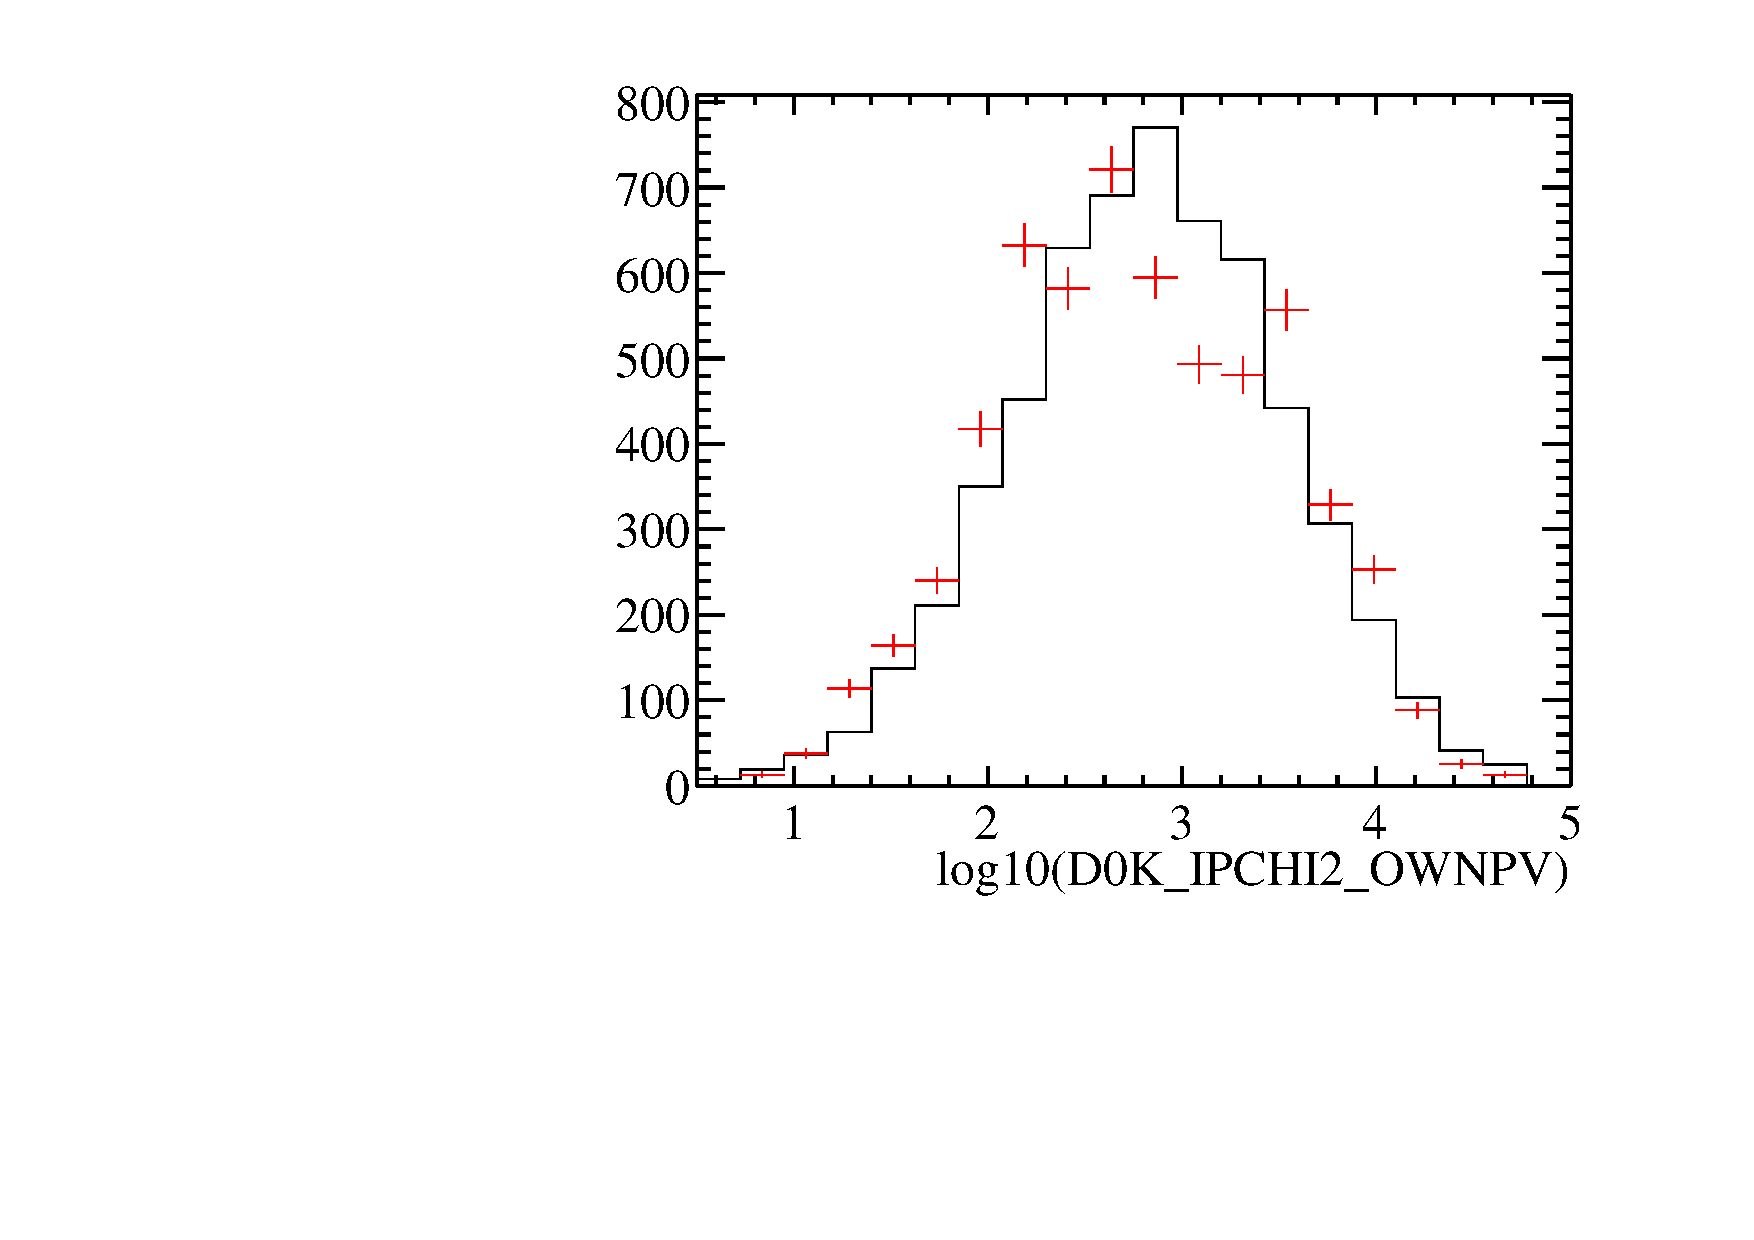
\includegraphics[width=0.3\textwidth]{ANA_resources/Plots/Monte_carlo/data_vs_MC/Kpi/log10(D0K_IPCHI2_OWNPV)_2012.pdf} & 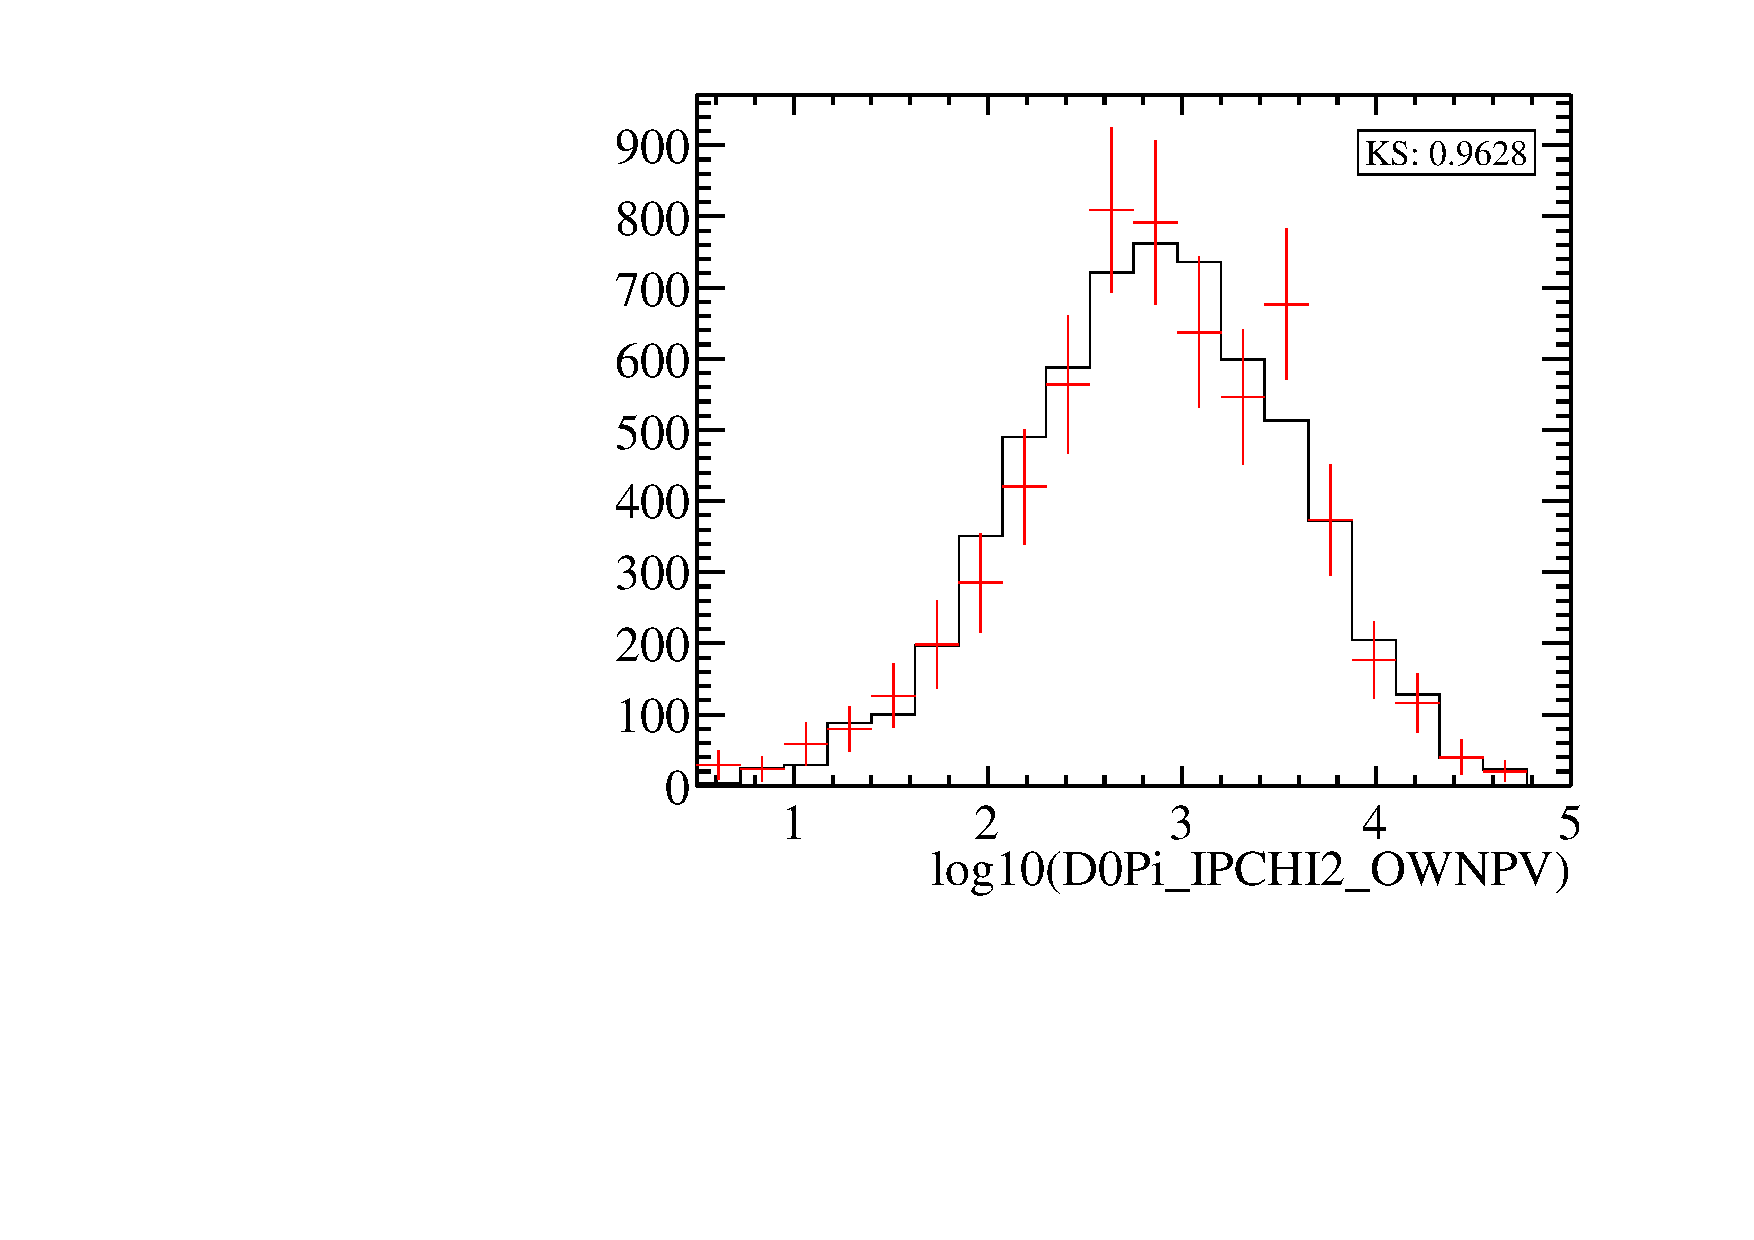
\includegraphics[width=0.3\textwidth]{ANA_resources/Plots/Monte_carlo/data_vs_MC/Kpi/log10(D0Pi_IPCHI2_OWNPV)_2012.pdf} & 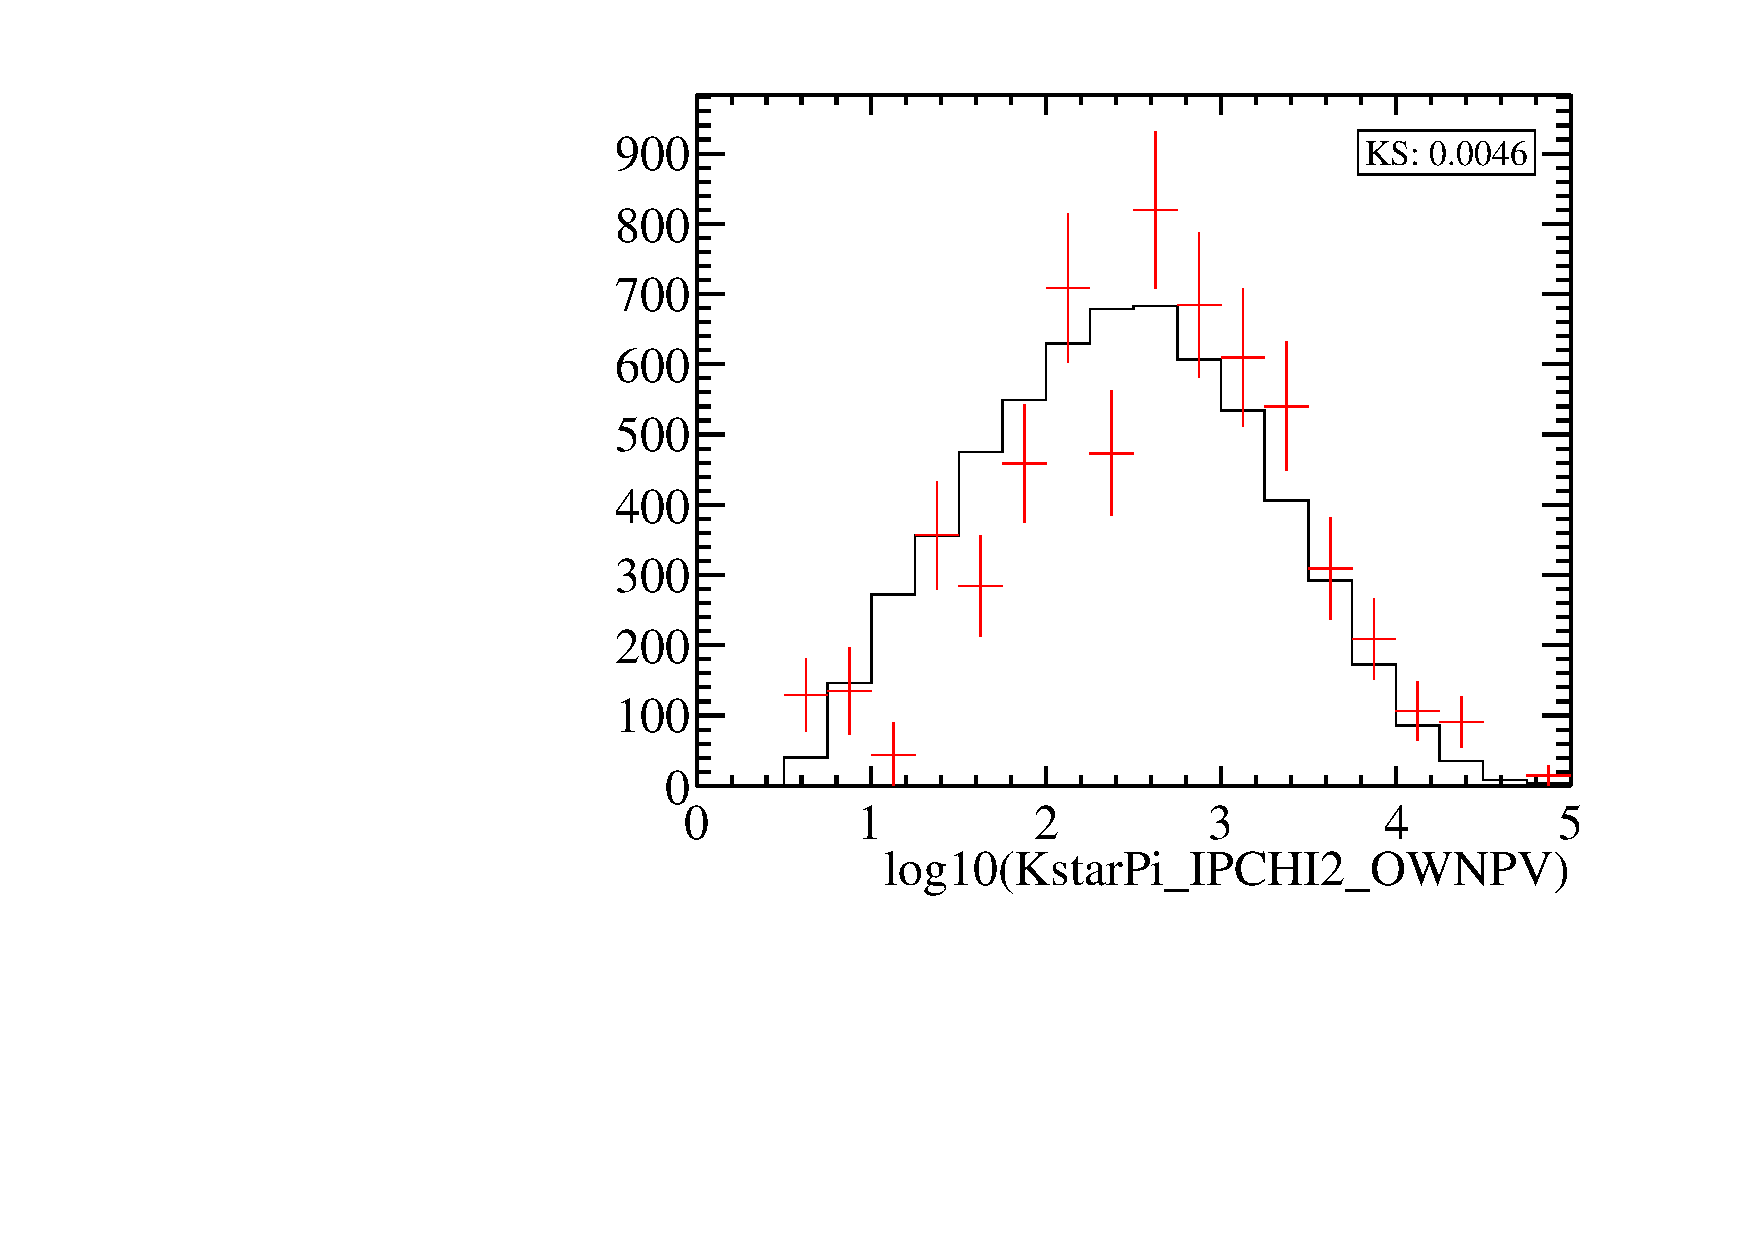
\includegraphics[width=0.3\textwidth]{ANA_resources/Plots/Monte_carlo/data_vs_MC/Kpi/log10(KstarPi_IPCHI2_OWNPV)_2012.pdf} \\
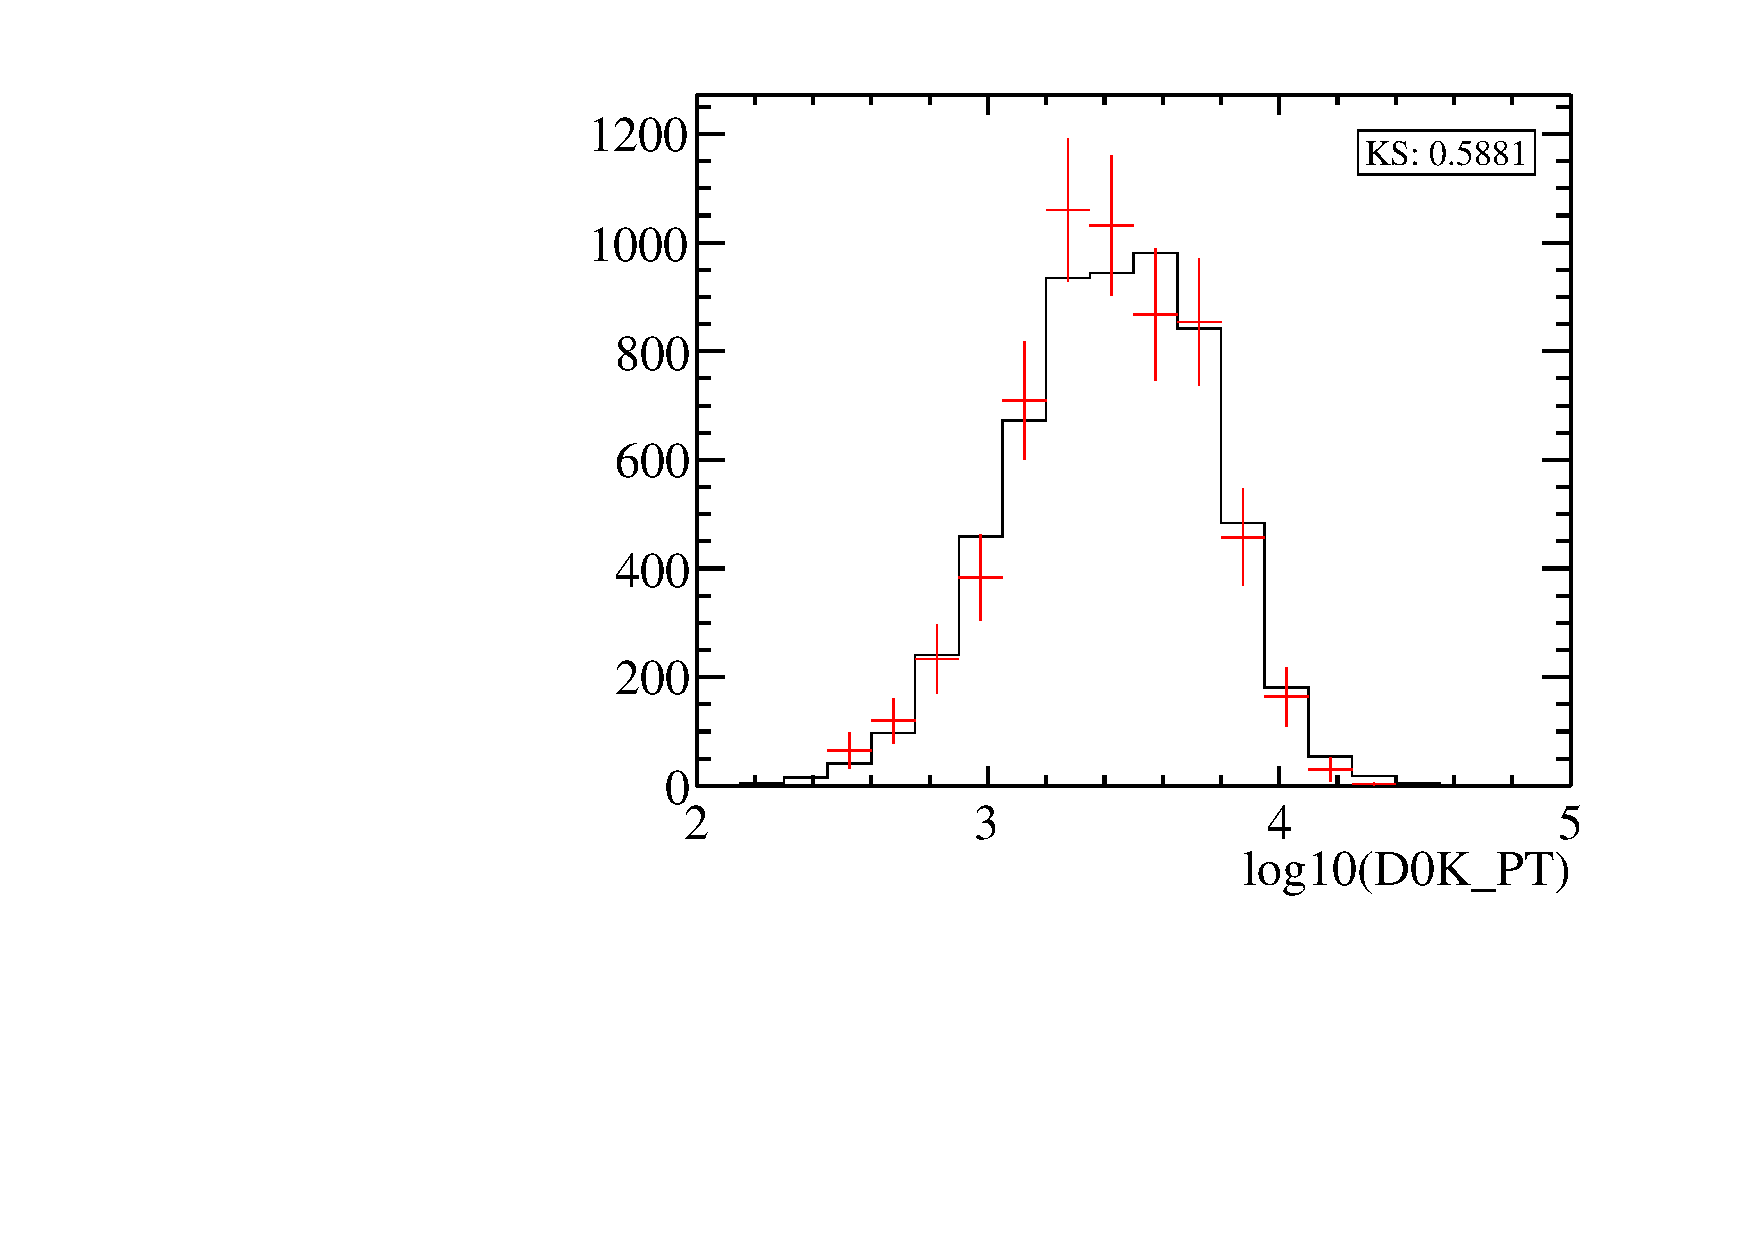
\includegraphics[width=0.3\textwidth]{ANA_resources/Plots/Monte_carlo/data_vs_MC/Kpi/log10(D0K_PT)_2012.pdf} & 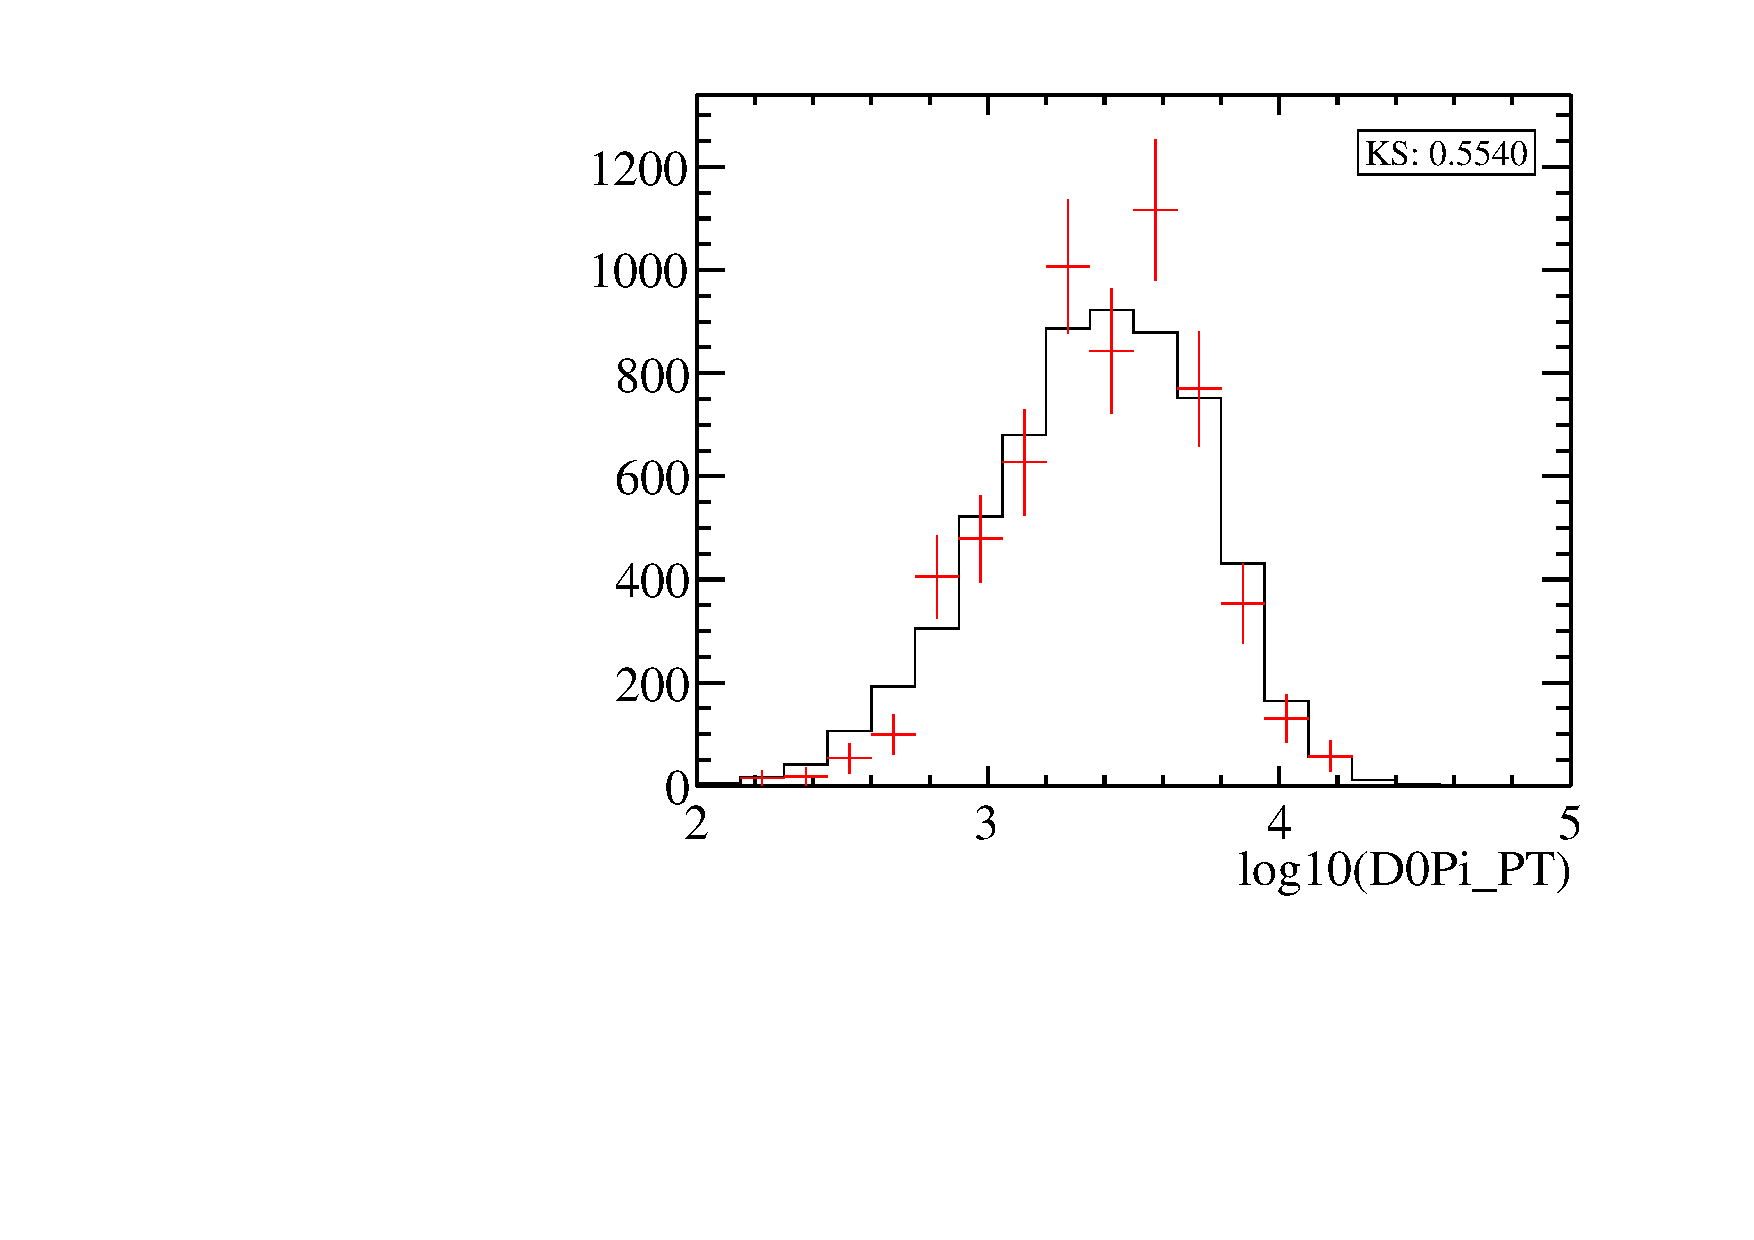
\includegraphics[width=0.3\textwidth]{ANA_resources/Plots/Monte_carlo/data_vs_MC/Kpi/log10(D0Pi_PT)_2012.pdf} & 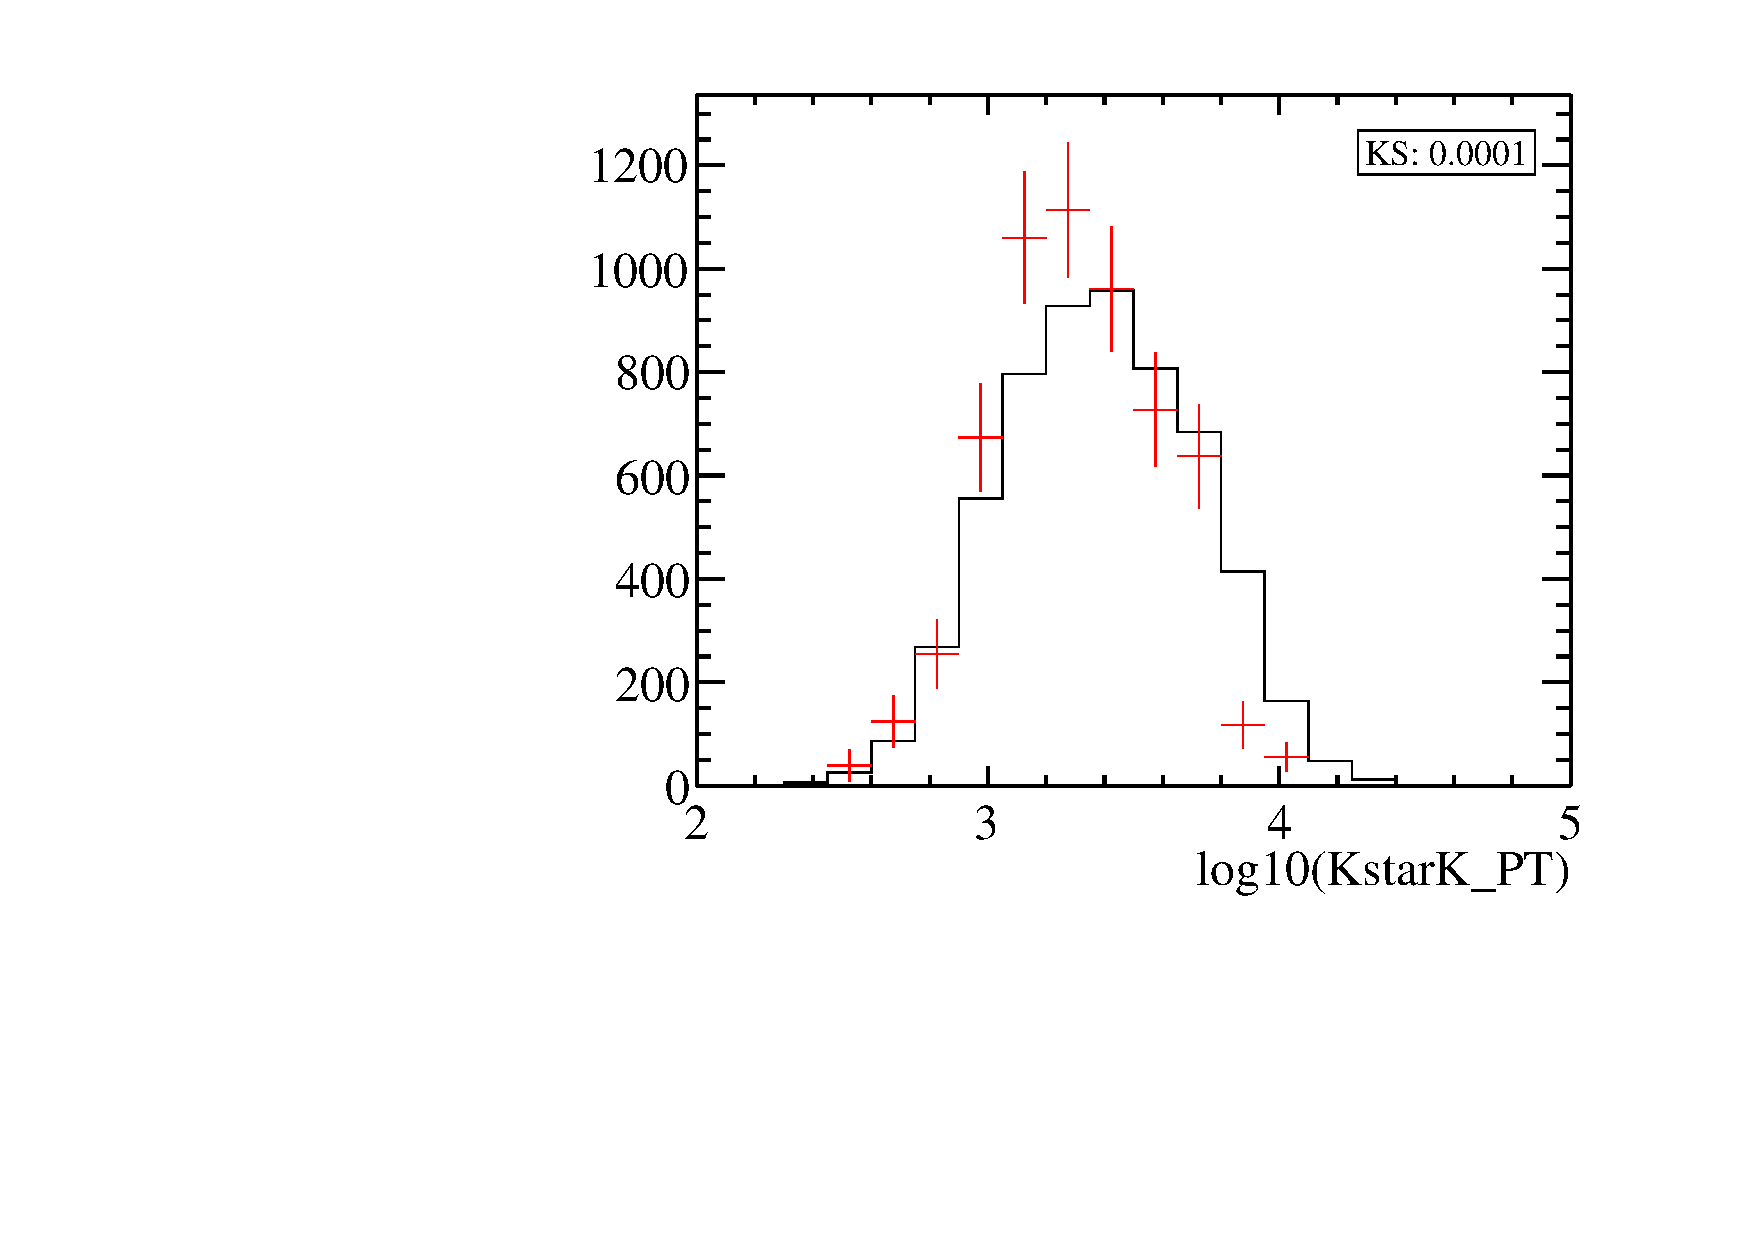
\includegraphics[width=0.3\textwidth]{ANA_resources/Plots/Monte_carlo/data_vs_MC/Kpi/log10(KstarK_PT)_2012.pdf} \\
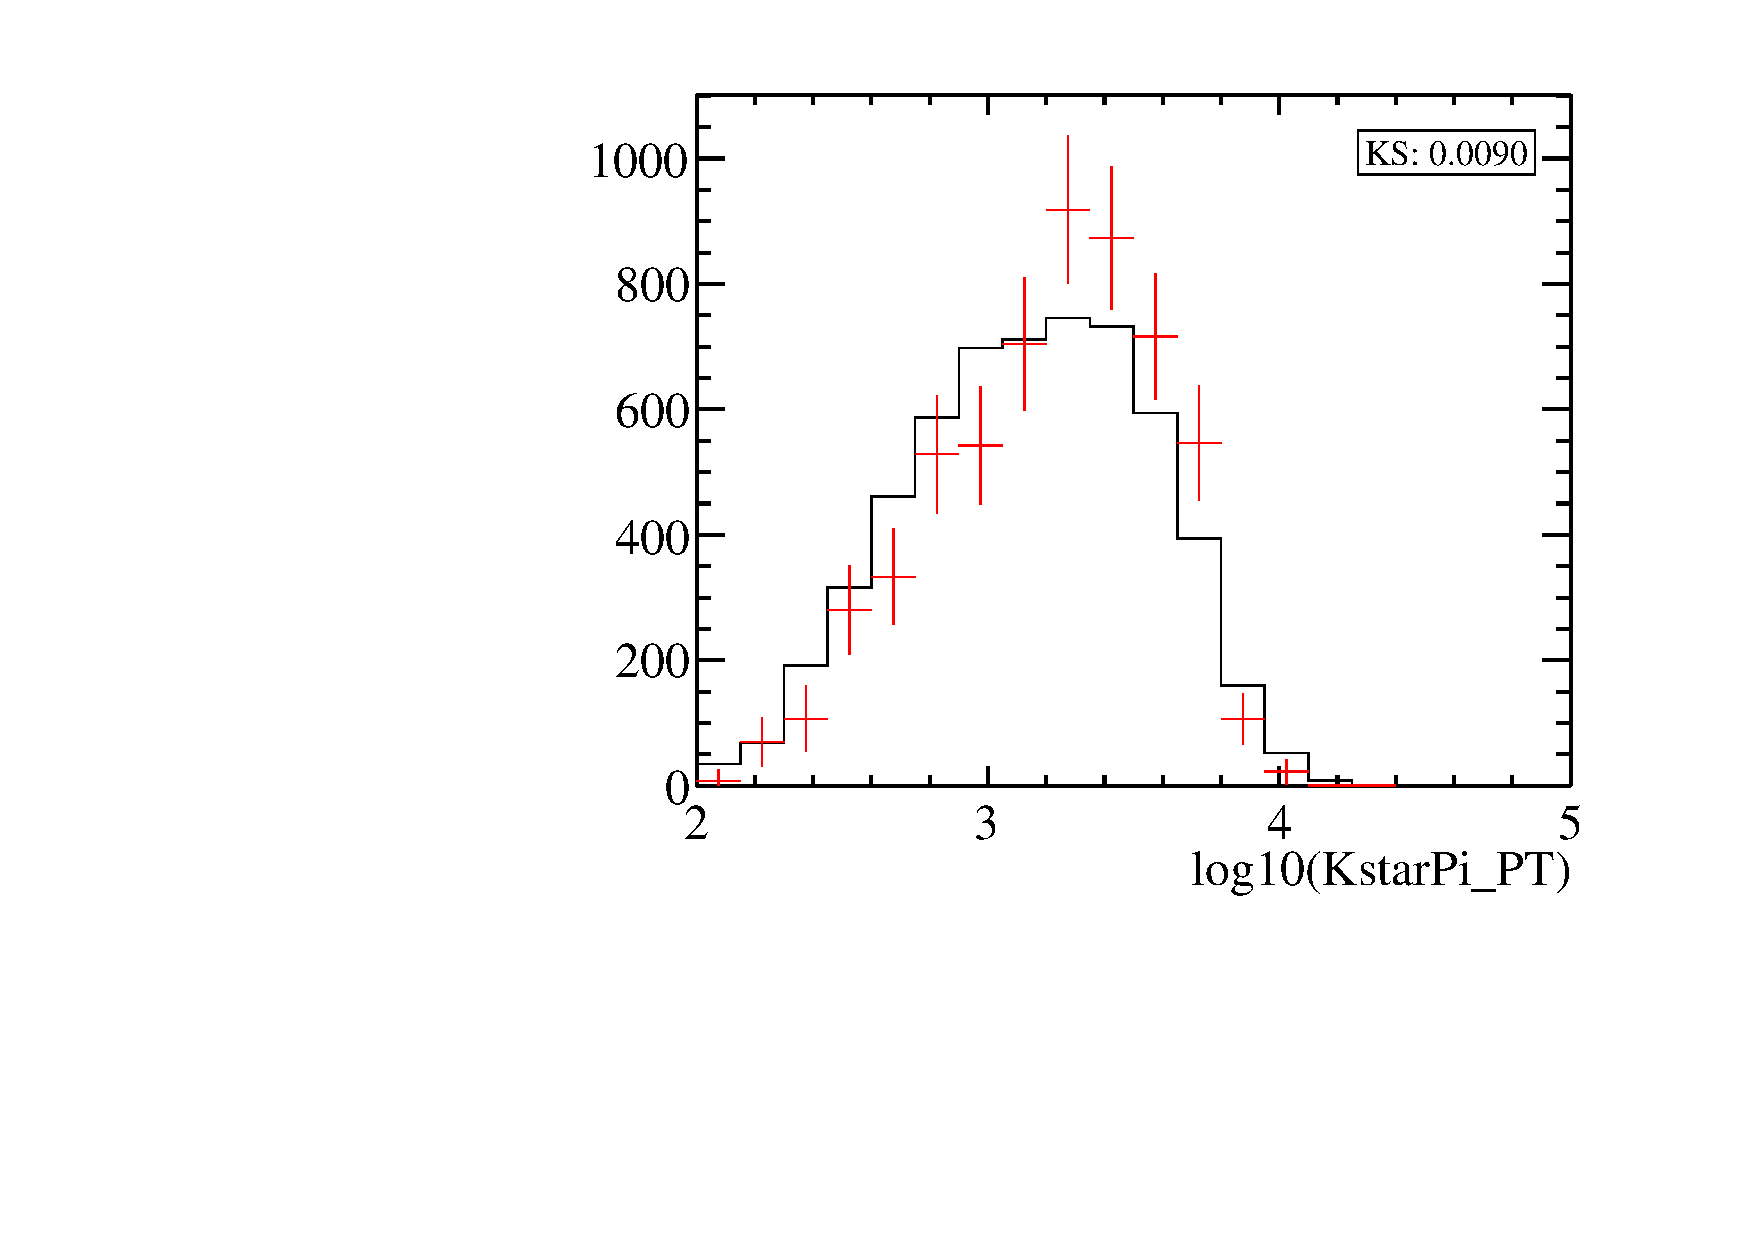
\includegraphics[width=0.3\textwidth]{ANA_resources/Plots/Monte_carlo/data_vs_MC/Kpi/log10(KstarPi_PT)_2012.pdf} & & \\
\end{tabular}
\caption{Comparison of 2012 data (red) and Monte Carlo (black) in the $K\pi$ mode for the variables used to train the $K\pi$ BDT.}
\label{fig:data_vs_MC_Kpi_2012}
\end{figure}
